% 名城大学理工学部情報工学科卒業研究発表会
% ・名城大学理工学研究科情報工学専攻公聴会
% アブストラクトサンプル
% Last Update: 2021/11/13

\documentclass[a4paper, 9pt]{jarticle}
\usepackage{ieabst}
\usepackage{newenum}
\usepackage[dvipdfmx]{graphicx}

%タイトルが長い場合は,勝手に改行されます.
%% 「\\」の挿入で任意の位置に改行を入れられます.
\題目{ヒント数17の数独パズルの効率的な生成に関する研究}
\学籍番号{223426015}
\氏名{長尾 卓}
\研究室{山本}
% 旭研究室 宇佐見研究室 亀谷研究室 川澄研究室 小中研究室
% 佐川研究室 鈴木研究室 高比良研究室 田中研究室 寺本研究室
% 中野研究室 野崎研究室 坂野研究室 水沼研究室 向井研究室
% 柳田研究室 山田(啓)研究室 山田(宗)研究室 山本研究室
% 吉川研究室 米澤研究室


%1ページに入りきらない場合は,下の数字を少し小さめに変更.
\renewcommand{\baselinestretch}{1}

\begin{document}
\small

\twocolumn[\vspace*{29mm}] %タイトルが2行の場合は29mm→36mmに.
\begin{論文概要}           %この行は消してはいけません

\section{はじめに}
数独パズルは,ペンシルパズルの一種である.
ペンシルパズルとは,問題に対して答えを徐々に鉛筆で書き込んでいき,
答えを導くようなパズルのことである.
ペンシルパズルには,数独パズルのほかにスリザーリンクや虫食い算などが
知られている.数独パズルは,与えられたヒント
(例:\figurename{\ref{fig:problem_and_answer}}左)から,
1から9の数字を用いて縦,横,$3 \times 3$ブロックの
どの数字にも重複させないように,マスを埋めていくパズルである.
\begin{figure}[b]
  \begin{minipage}[b]{0.49\linewidth}
    \centering
    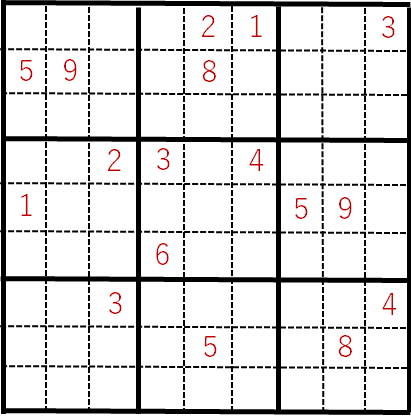
\includegraphics[width=3.5cm]{prob.png}
  \end{minipage}
  \begin{minipage}[b]{0.49\linewidth}
    \centering
    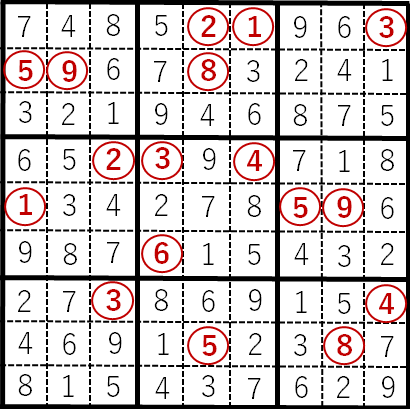
\includegraphics[width=3.5cm]{ans.png}
  \end{minipage}
  \caption{17個のヒントによる数独パズルの問題(左)とその解(右).}
  \label{fig:problem_and_answer}
\end{figure}
\figurename{\ref{fig:problem_and_answer}}左で与えられる問題の
答えは\figurename{\ref{fig:problem_and_answer}}右である.
また,1つの問題から得られる最終盤面はただ1通りである必要がある.
以降,数独パズルの最終盤面を「解」と表す.
本研究には先行研究 \cite{previous_research} がある.
先行研究の目的は,ヒント数が少ない
数独パズルの問題を確率的に効率よく生成することである.
先行研究が提案するヒント生成アルゴリズムの
ヒント数17の問題生成割合は約5\%であり,
1つの問題を生成する平均時間
\footnote{プログラムの実行環境は以下の通りである: 
OS:Linux Ubuntu 16.04.7,
CPU:Intel(R) Xeon(R) CPU E5-2640 v4 @ 2.40GHz,
メモリ:64G,
コンパイラ:gcc5.4.0.
}
は約105分であった.
なお,数独パズルにおけるヒント数の下限は17個であることが 
\cite{seventeen_hints} により証明されている.
先行研究により,確率的にヒント数17の問題を生成できることが分かったため,
本研究ではヒント数17の問題を効率よく生成することを目的とした.
本研究が提案するヒント生成アルゴリズムは,先行研究の
ヒント生成アルゴリズムを改良したものである.
提案するヒント生成アルゴリズムは
ヒント数17の問題を約93\%の確率で生成し,
先行研究と同環境で1つの問題を生成する平均時間は約11分であった.

\section{本研究で用いる手法}
本研究ではシミュレイテッド・アニーリング(SA) \cite{sa} と,
ビームサーチ(BS) \cite{beam_search},Algorithm X \cite{AX} の
3つの手法を用いる.以下にそれらの説明をする.

SAは目的の定常分布をもつマルコフ連鎖 \cite{mcmc} を
安定して構成するヒューリスティックなアルゴリズムである.
マルコフ連鎖上のある状態からランダムな近傍状態に遷移させる
ことを繰り返し,マルコフ連鎖を定常状態にした後に,
SAのパラメータである内部温度$T$を微減させて
定常分布を目的の定常分布へ緩く変化させる.
以上を繰り返すことで,目的の定常分布をもつマルコフ連鎖を構成していく.
そして,目的の定常分布を得るまでに,
得たい状態をサンプリングすることが可能である.
一般的なSAは,ある状態の出現確率をボルツマン因子により決定し,
近傍状態への遷移にはメトロポリス法 \cite{sa} を用いる.
本研究もボルツマン因子やメトロポリス法を用いる.

BSは,木構造上の根からスタートする$w$本のパスを考えて,
それらのパスを同時に葉の方向に伸ばしながら評価値がより良いノードを
探索するヒューリスティックな探索アルゴリズムである.
BSの性質は$w$によって大きく変化する.
$w$が大きい場合は,空間的計算量と時間的計算量の両方が大きくなる.
一方で,$w$が小さい場合は,最適解や最適解に近いノードへのパスが
途中で絶たれる可能性が大きくなる.

AXは,集合$S$と複数の部分集合$s$をもつ厳密被覆問題をバックトラックで
効率よく解くアルゴリズムである.ある時点までに選択してきた全ての$s$と
互いに素の$s$のみを保持し,保持している部分集合から適切に$s$を選択
することを再帰的に繰り返す.保持している部分集合のみでは
$S$の要素をカバーできないと判断した場合に,効率よく枝狩りを行うため効率がよい.

\section{先行研究のヒント生成アルゴリズム}
本研究が提案するヒント生成アルゴリズムは \cite{previous_research} の方法を
改善したものである.先行研究のヒント生成アルゴリズムは,
まず,ヒント集合$H^{(0)} = \emptyset$を用意する.
$H^{(0)}$の右肩の数字が表記されている場合は,
ヒント集合$H$のサイズを表す.
次に,適切なヒント$h$を$H$に添加していき,
$H$から得られる解の集合の大きさ$|S(H)|$を徐々に減少させていく.
$h$はマスの位置$p$と数字$n$の組である.
適切な$h$とは,$H^{(i)}$に添加して得られる$H^{(i+1)}$の
$|S(H)|$が最小となる$h$のことである.
最終的には,$|S(H)| = 1$となるまで$h$を$H$に添加して問題を生成する.
$h$の選択方法は,$H$から$S(H)$を得て,得た解に出現した場所と
数字の組である複数の要素のうち最も出現回数が少ない要素を$h$とする.
なお,$H$から$S(H)$を得るためには,
バックトラック(BT)を用いる.
一方で,$H^{(i)} ~ (i < 14)$は十分に解集合の大きさが減少しておらず,
BTで解を列挙することは効率が悪い.
そのため,シミュレイテッド・アニーリング(SA)を用いることで
$H^{(i)}$から得られる解を偏りなく等確率に多く生成することを行い,
確率的に$h$を選択する.

\section{先行研究のヒント生成アルゴリズムに加えた改良}
前述したように,本研究が提案するヒント生成アルゴリズムは,
先行研究のヒント生成アルゴリズムを改良したものである.
改良した点は主に4点であり,2点はヒント数17の問題生成割合を高めるための
改良で,残りの2点はヒント生成の高速化のために行った改良である.
ヒント数17の問題生成割合の向上のための改良1点目は,
生成した$H^{(14)}$に3つの$h$をまとめて添加するようにした点である.
これにより,生成した$H^{(14)}$があるヒント数17の問題の部分集合である
場合は,必ずそのヒント数17の問題を生成できるようになる.
先行研究のヒント生成アルゴリズムにこの改良を加えた場合の
ヒント数別の問題生成割合は\figurename{\ref{fig:prob_under_add_3hints}}
のように変化し,ヒント数17の問題生成割合は約5\%から約10\%に上昇した.
\begin{figure}[bt]
  \centering
  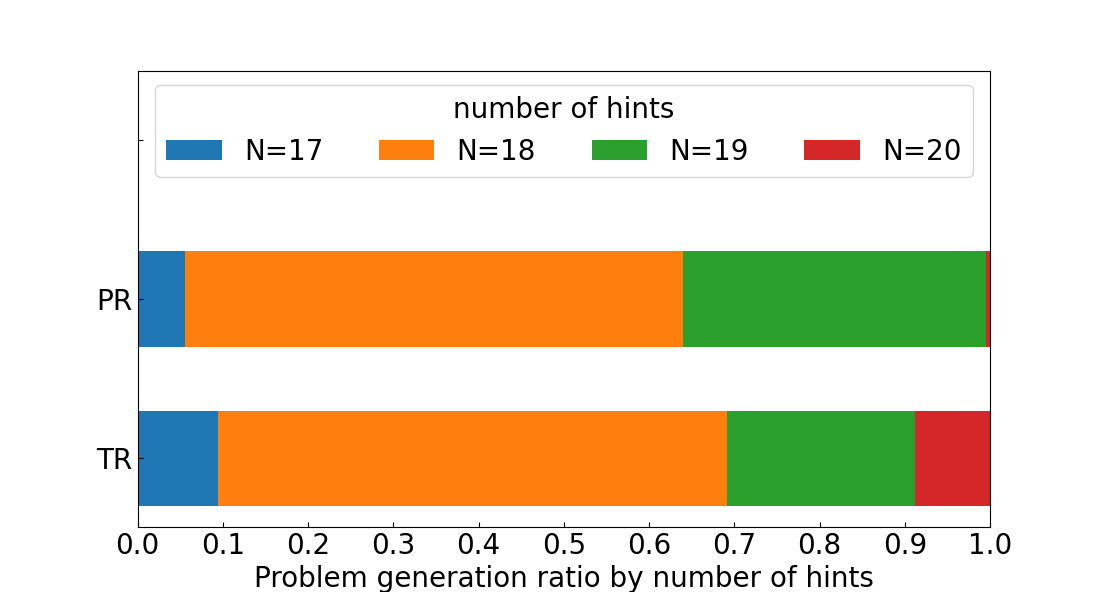
\includegraphics[keepaspectratio, scale=0.25]{prob_under_add_3hints.png}
  \caption{先行研究のヒント生成アルゴリズムに$H^{(14)}$に3つのヒントをまとめて
  添加する変更を加えたアルゴリズムの問題生成割合.
  PRが先行研究であり,3Rが本変更を加えたアルゴリズムを表している.} 
  \label{fig:prob_under_add_3hints}
\end{figure}
2点目は,生成していく$H^{(i)}$の解集合を柔軟に減少させていくために,
最も解集合が小さい$w$個の$H^{(i)}$を
保持していくBSを用いた点である \cite{nagao}.
生成した$H^{(14)}$の解集合が小さいときほど,
$H^{(14)}$に3つのヒントを添加する場合に,
ヒント数17の問題を生成しやすくなることが実験により分かっている.
本研究で行うBSには一般的なBSにはないパラメータがあり,
1つの$H^{(i)}$から生成する$H^{(i+1)}$の個数の上限$\rho$を設けている.
パラメータ$\rho$は,解集合が減少していきずらい$H^{(i)}$から生成された
$H^{(i+1)}$のみをBSで保持することを避ける目的がある.
\begin{figure}[bt]
  \centering
  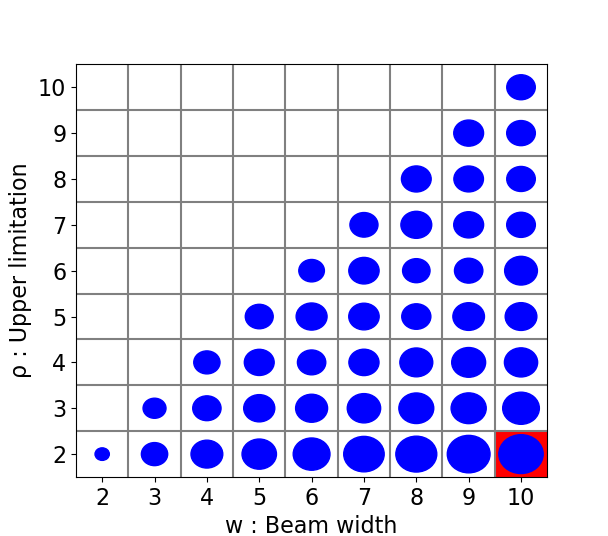
\includegraphics[keepaspectratio, scale=0.4]{best_beam_width_and_rho.png}
  \caption{ビーム幅$w~(2 \leq w \leq 10)$と上限$\rho~(2 \leq \rho \leq w)$の組み合わせ
  により,$B^{(14)}$に含まれる最も解集合が小さい$H^{(14)}_j$の
  解集合の大きさが$U = 160,000$以下になる確率を円の大きさで表した図.
  $w$は横軸で表し,$\rho$は縦軸で表す.
  最も生成割合が高かった$w$と$\rho$の組を赤色で表している.} 
  \label{fig:best_beam_width_and_rho}
\end{figure}
ヒント生成の高速化のための改良1点目は,
$H^{(i)} ~ (i \geq 14)$から解集合を得るためにBTではなく,
Algorithm Xを用いるようにした点である.
Algorithm Xは厳密被覆問題を効率よく解くことができる
アルゴリズムであり,数独パズルは厳密被覆問題として定義することができる
ことから,本研究はBTではなくAlgorithm Xを用いることとした.
この変更により,$H^{(14)}$にまとめて添加する3つのヒントの選択時間は
約$66 \sim 80$\%ほど短縮した.
2点目は,$H$から解をサンプリングするSAにおける,
近傍状態の決定方法を変更した点である.
先行研究のSAは,ランダムに行を選択し,選択した行内のヒント以外の2マスの
数字を交換するように遷移先の近傍状態を決定する.
ただし,初めに$H$を考慮して全行に1から9が無作為に
書き込まれた初期盤面から遷移を行うようにする.
一方で,本研究のSAは,ランダムに$3 \times 3$ブロックを選択し,
選択したブロック内のヒント以外の2マスの数字を交換するように遷移先の近傍状態を決定する.
ただし,初めに$H$を考慮して全ブロックに1から9が無作為に
書き込まれた初期盤面から遷移を行う.
この変更により,SAの解のサンプリング効率が約5倍向上した.

\begin{thebibliography}{10}

  \bibitem{previous_research}
  古川 湧:ヒントの少ない数独パズルの生成に関する研究.$2020$年度名城大学大学院理工学研究科修士論文(2021).
  
  \bibitem{nagao}
  長尾 卓:ビームサーチを用いたヒント数17の数独パズルの効率的な生成について.
  {\it ゲームプログラミングワークショップ2022論文集},pp. 96--103 (2022).
  
  \bibitem{seventeen_hints}
  G. McGuire, B. Tugemann, and G. Civario:
  There is no 16-clue Sudoku: Solving the Sudoku minimum number of clues problem via hitting set enumeration.
  {\it Experimental Mathematics}, 23:2, pp. 190--217 (2014).

  \bibitem{sa}
  Bruce E. Rosen,中野 良平:シミュレーテッドアニーリング:ー基礎と最新技術ー,
  人工知能学会誌,Vol.9,No.3,pp.365--372(1994).
  
  \bibitem{beam_search}
  Y. Inoue and S. Minato: Acceleration of ZDD Construction for Subgraph 
  Enumeration via Path-width Optimization. TCS Technical Report, 
  TSC-TR-A-16-80, (2016).

  \bibitem{AX}
  D. E. Knuth: Dancing links. 
  {\it Millennial Perspectives in Computer Science}, pp. 187--214 (2000).

  \bibitem{mcmc}
  Berg, B.: Markov Chain Monte Carlo Simulations and Their Statistical
  Analysis. World Scientific Publishing Co. Pte. Ltd. (2004).
  
\end{thebibliography}

\end{論文概要} %この行は消してはいけません
\end{document}
